% Created by tikzDevice version 0.12 on 2019-02-08 11:09:24
% !TEX encoding = UTF-8 Unicode
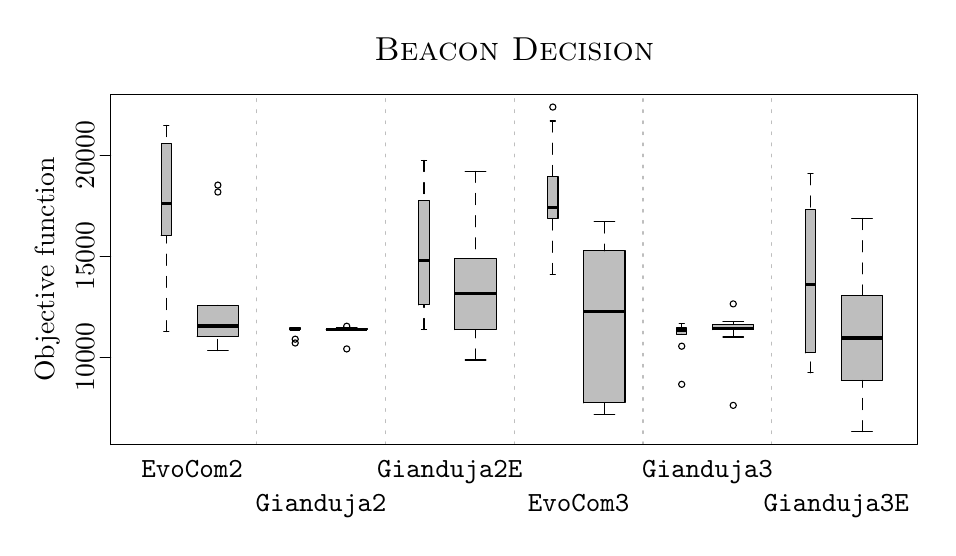
\begin{tikzpicture}[x=1pt,y=1pt]
\definecolor{fillColor}{RGB}{255,255,255}
\path[use as bounding box,fill=fillColor,fill opacity=0.00] (0,0) rectangle (325.21,180.67);
\begin{scope}
\path[clip] ( 30.00, 30.00) rectangle (321.61,156.67);
\definecolor{fillColor}{RGB}{190,190,190}

\path[fill=fillColor] ( 48.25,105.50) --
	( 51.97,105.50) --
	( 51.97,138.71) --
	( 48.25,138.71) --
	cycle;
\definecolor{drawColor}{RGB}{0,0,0}

\path[draw=drawColor,line width= 1.2pt,line join=round] ( 48.25,117.05) -- ( 51.97,117.05);

\path[draw=drawColor,line width= 0.4pt,dash pattern=on 4pt off 4pt ,line join=round,line cap=round] ( 50.11, 70.81) -- ( 50.11,105.50);

\path[draw=drawColor,line width= 0.4pt,dash pattern=on 4pt off 4pt ,line join=round,line cap=round] ( 50.11,145.31) -- ( 50.11,138.71);

\path[draw=drawColor,line width= 0.4pt,line join=round,line cap=round] ( 49.18, 70.81) -- ( 51.04, 70.81);

\path[draw=drawColor,line width= 0.4pt,line join=round,line cap=round] ( 49.18,145.31) -- ( 51.04,145.31);

\path[draw=drawColor,line width= 0.4pt,line join=round,line cap=round] ( 48.25,105.50) --
	( 51.97,105.50) --
	( 51.97,138.71) --
	( 48.25,138.71) --
	( 48.25,105.50);

\path[fill=fillColor] ( 61.28, 69.04) --
	( 76.18, 69.04) --
	( 76.18, 80.34) --
	( 61.28, 80.34) --
	cycle;

\path[draw=drawColor,line width= 1.2pt,line join=round] ( 61.28, 72.87) -- ( 76.18, 72.87);

\path[draw=drawColor,line width= 0.4pt,dash pattern=on 4pt off 4pt ,line join=round,line cap=round] ( 68.73, 64.03) -- ( 68.73, 69.04);

\path[draw=drawColor,line width= 0.4pt,dash pattern=on 4pt off 4pt ,line join=round,line cap=round] ( 68.73, 80.34) -- ( 68.73, 80.34);

\path[draw=drawColor,line width= 0.4pt,line join=round,line cap=round] ( 65.01, 64.03) -- ( 72.46, 64.03);

\path[draw=drawColor,line width= 0.4pt,line join=round,line cap=round] ( 65.01, 80.34) -- ( 72.46, 80.34);

\path[draw=drawColor,line width= 0.4pt,line join=round,line cap=round] ( 61.28, 69.04) --
	( 76.18, 69.04) --
	( 76.18, 80.34) --
	( 61.28, 80.34) --
	( 61.28, 69.04);

\path[draw=drawColor,line width= 0.4pt,line join=round,line cap=round] ( 68.73,123.78) circle (  1.12);

\path[draw=drawColor,line width= 0.4pt,line join=round,line cap=round] ( 68.73,121.27) circle (  1.12);

\path[fill=fillColor] ( 94.80, 71.46) --
	( 98.53, 71.46) --
	( 98.53, 72.13) --
	( 94.80, 72.13) --
	cycle;

\path[draw=drawColor,line width= 1.2pt,line join=round] ( 94.80, 71.58) -- ( 98.53, 71.58);

\path[draw=drawColor,line width= 0.4pt,dash pattern=on 4pt off 4pt ,line join=round,line cap=round] ( 96.67, 71.46) -- ( 96.67, 71.46);

\path[draw=drawColor,line width= 0.4pt,dash pattern=on 4pt off 4pt ,line join=round,line cap=round] ( 96.67, 72.16) -- ( 96.67, 72.13);

\path[draw=drawColor,line width= 0.4pt,line join=round,line cap=round] ( 95.73, 71.46) -- ( 97.60, 71.46);

\path[draw=drawColor,line width= 0.4pt,line join=round,line cap=round] ( 95.73, 72.16) -- ( 97.60, 72.16);

\path[draw=drawColor,line width= 0.4pt,line join=round,line cap=round] ( 94.80, 71.46) --
	( 98.53, 71.46) --
	( 98.53, 72.13) --
	( 94.80, 72.13) --
	( 94.80, 71.46);

\path[draw=drawColor,line width= 0.4pt,line join=round,line cap=round] ( 96.67, 66.73) circle (  1.12);

\path[draw=drawColor,line width= 0.4pt,line join=round,line cap=round] ( 96.67, 68.11) circle (  1.12);

\path[fill=fillColor] (107.84, 71.46) --
	(122.74, 71.46) --
	(122.74, 71.99) --
	(107.84, 71.99) --
	cycle;

\path[draw=drawColor,line width= 1.2pt,line join=round] (107.84, 71.58) -- (122.74, 71.58);

\path[draw=drawColor,line width= 0.4pt,dash pattern=on 4pt off 4pt ,line join=round,line cap=round] (115.29, 71.35) -- (115.29, 71.46);

\path[draw=drawColor,line width= 0.4pt,dash pattern=on 4pt off 4pt ,line join=round,line cap=round] (115.29, 72.21) -- (115.29, 71.99);

\path[draw=drawColor,line width= 0.4pt,line join=round,line cap=round] (111.56, 71.35) -- (119.01, 71.35);

\path[draw=drawColor,line width= 0.4pt,line join=round,line cap=round] (111.56, 72.21) -- (119.01, 72.21);

\path[draw=drawColor,line width= 0.4pt,line join=round,line cap=round] (107.84, 71.46) --
	(122.74, 71.46) --
	(122.74, 71.99) --
	(107.84, 71.99) --
	(107.84, 71.46);

\path[draw=drawColor,line width= 0.4pt,line join=round,line cap=round] (115.29, 64.59) circle (  1.12);

\path[draw=drawColor,line width= 0.4pt,line join=round,line cap=round] (115.29, 72.78) circle (  1.12);

\path[fill=fillColor] (141.36, 80.48) --
	(145.08, 80.48) --
	(145.08,118.27) --
	(141.36,118.27) --
	cycle;

\path[draw=drawColor,line width= 1.2pt,line join=round] (141.36, 96.51) -- (145.08, 96.51);

\path[draw=drawColor,line width= 0.4pt,dash pattern=on 4pt off 4pt ,line join=round,line cap=round] (143.22, 71.58) -- (143.22, 80.48);

\path[draw=drawColor,line width= 0.4pt,dash pattern=on 4pt off 4pt ,line join=round,line cap=round] (143.22,132.68) -- (143.22,118.27);

\path[draw=drawColor,line width= 0.4pt,line join=round,line cap=round] (142.29, 71.58) -- (144.15, 71.58);

\path[draw=drawColor,line width= 0.4pt,line join=round,line cap=round] (142.29,132.68) -- (144.15,132.68);

\path[draw=drawColor,line width= 0.4pt,line join=round,line cap=round] (141.36, 80.48) --
	(145.08, 80.48) --
	(145.08,118.27) --
	(141.36,118.27) --
	(141.36, 80.48);

\path[fill=fillColor] (154.39, 71.58) --
	(169.29, 71.58) --
	(169.29, 97.27) --
	(154.39, 97.27) --
	cycle;

\path[draw=drawColor,line width= 1.2pt,line join=round] (154.39, 84.72) -- (169.29, 84.72);

\path[draw=drawColor,line width= 0.4pt,dash pattern=on 4pt off 4pt ,line join=round,line cap=round] (161.84, 60.58) -- (161.84, 71.58);

\path[draw=drawColor,line width= 0.4pt,dash pattern=on 4pt off 4pt ,line join=round,line cap=round] (161.84,128.74) -- (161.84, 97.27);

\path[draw=drawColor,line width= 0.4pt,line join=round,line cap=round] (158.12, 60.58) -- (165.57, 60.58);

\path[draw=drawColor,line width= 0.4pt,line join=round,line cap=round] (158.12,128.74) -- (165.57,128.74);

\path[draw=drawColor,line width= 0.4pt,line join=round,line cap=round] (154.39, 71.58) --
	(169.29, 71.58) --
	(169.29, 97.27) --
	(154.39, 97.27) --
	(154.39, 71.58);

\path[fill=fillColor] (187.91,111.80) --
	(191.64,111.80) --
	(191.64,127.04) --
	(187.91,127.04) --
	cycle;

\path[draw=drawColor,line width= 1.2pt,line join=round] (187.91,115.65) -- (191.64,115.65);

\path[draw=drawColor,line width= 0.4pt,dash pattern=on 4pt off 4pt ,line join=round,line cap=round] (189.77, 91.52) -- (189.77,111.80);

\path[draw=drawColor,line width= 0.4pt,dash pattern=on 4pt off 4pt ,line join=round,line cap=round] (189.77,146.93) -- (189.77,127.04);

\path[draw=drawColor,line width= 0.4pt,line join=round,line cap=round] (188.84, 91.52) -- (190.70, 91.52);

\path[draw=drawColor,line width= 0.4pt,line join=round,line cap=round] (188.84,146.93) -- (190.70,146.93);

\path[draw=drawColor,line width= 0.4pt,line join=round,line cap=round] (187.91,111.80) --
	(191.64,111.80) --
	(191.64,127.04) --
	(187.91,127.04) --
	(187.91,111.80);

\path[draw=drawColor,line width= 0.4pt,line join=round,line cap=round] (189.77,151.98) circle (  1.12);

\path[fill=fillColor] (200.95, 45.12) --
	(215.84, 45.12) --
	(215.84,100.06) --
	(200.95,100.06) --
	cycle;

\path[draw=drawColor,line width= 1.2pt,line join=round] (200.95, 78.06) -- (215.84, 78.06);

\path[draw=drawColor,line width= 0.4pt,dash pattern=on 4pt off 4pt ,line join=round,line cap=round] (208.40, 40.92) -- (208.40, 45.12);

\path[draw=drawColor,line width= 0.4pt,dash pattern=on 4pt off 4pt ,line join=round,line cap=round] (208.40,110.48) -- (208.40,100.06);

\path[draw=drawColor,line width= 0.4pt,line join=round,line cap=round] (204.67, 40.92) -- (212.12, 40.92);

\path[draw=drawColor,line width= 0.4pt,line join=round,line cap=round] (204.67,110.48) -- (212.12,110.48);

\path[draw=drawColor,line width= 0.4pt,line join=round,line cap=round] (200.95, 45.12) --
	(215.84, 45.12) --
	(215.84,100.06) --
	(200.95,100.06) --
	(200.95, 45.12);

\path[fill=fillColor] (234.47, 69.86) --
	(238.19, 69.86) --
	(238.19, 72.13) --
	(234.47, 72.13) --
	cycle;

\path[draw=drawColor,line width= 1.2pt,line join=round] (234.47, 71.34) -- (238.19, 71.34);

\path[draw=drawColor,line width= 0.4pt,dash pattern=on 4pt off 4pt ,line join=round,line cap=round] (236.33, 69.86) -- (236.33, 69.86);

\path[draw=drawColor,line width= 0.4pt,dash pattern=on 4pt off 4pt ,line join=round,line cap=round] (236.33, 73.62) -- (236.33, 72.13);

\path[draw=drawColor,line width= 0.4pt,line join=round,line cap=round] (235.40, 69.86) -- (237.26, 69.86);

\path[draw=drawColor,line width= 0.4pt,line join=round,line cap=round] (235.40, 73.62) -- (237.26, 73.62);

\path[draw=drawColor,line width= 0.4pt,line join=round,line cap=round] (234.47, 69.86) --
	(238.19, 69.86) --
	(238.19, 72.13) --
	(234.47, 72.13) --
	(234.47, 69.86);

\path[draw=drawColor,line width= 0.4pt,line join=round,line cap=round] (236.33, 51.79) circle (  1.12);

\path[draw=drawColor,line width= 0.4pt,line join=round,line cap=round] (236.33, 65.57) circle (  1.12);

\path[fill=fillColor] (247.50, 71.58) --
	(262.40, 71.58) --
	(262.40, 73.56) --
	(247.50, 73.56) --
	cycle;

\path[draw=drawColor,line width= 1.2pt,line join=round] (247.50, 71.95) -- (262.40, 71.95);

\path[draw=drawColor,line width= 0.4pt,dash pattern=on 4pt off 4pt ,line join=round,line cap=round] (254.95, 68.89) -- (254.95, 71.58);

\path[draw=drawColor,line width= 0.4pt,dash pattern=on 4pt off 4pt ,line join=round,line cap=round] (254.95, 74.43) -- (254.95, 73.56);

\path[draw=drawColor,line width= 0.4pt,line join=round,line cap=round] (251.23, 68.89) -- (258.67, 68.89);

\path[draw=drawColor,line width= 0.4pt,line join=round,line cap=round] (251.23, 74.43) -- (258.67, 74.43);

\path[draw=drawColor,line width= 0.4pt,line join=round,line cap=round] (247.50, 71.58) --
	(262.40, 71.58) --
	(262.40, 73.56) --
	(247.50, 73.56) --
	(247.50, 71.58);

\path[draw=drawColor,line width= 0.4pt,line join=round,line cap=round] (254.95, 44.19) circle (  1.12);

\path[draw=drawColor,line width= 0.4pt,line join=round,line cap=round] (254.95, 80.86) circle (  1.12);

\path[fill=fillColor] (281.02, 63.19) --
	(284.74, 63.19) --
	(284.74,114.93) --
	(281.02,114.93) --
	cycle;

\path[draw=drawColor,line width= 1.2pt,line join=round] (281.02, 87.89) -- (284.74, 87.89);

\path[draw=drawColor,line width= 0.4pt,dash pattern=on 4pt off 4pt ,line join=round,line cap=round] (282.88, 55.91) -- (282.88, 63.19);

\path[draw=drawColor,line width= 0.4pt,dash pattern=on 4pt off 4pt ,line join=round,line cap=round] (282.88,127.84) -- (282.88,114.93);

\path[draw=drawColor,line width= 0.4pt,line join=round,line cap=round] (281.95, 55.91) -- (283.81, 55.91);

\path[draw=drawColor,line width= 0.4pt,line join=round,line cap=round] (281.95,127.84) -- (283.81,127.84);

\path[draw=drawColor,line width= 0.4pt,line join=round,line cap=round] (281.02, 63.19) --
	(284.74, 63.19) --
	(284.74,114.93) --
	(281.02,114.93) --
	(281.02, 63.19);

\path[fill=fillColor] (294.05, 53.21) --
	(308.95, 53.21) --
	(308.95, 84.00) --
	(294.05, 84.00) --
	cycle;

\path[draw=drawColor,line width= 1.2pt,line join=round] (294.05, 68.59) -- (308.95, 68.59);

\path[draw=drawColor,line width= 0.4pt,dash pattern=on 4pt off 4pt ,line join=round,line cap=round] (301.50, 34.69) -- (301.50, 53.21);

\path[draw=drawColor,line width= 0.4pt,dash pattern=on 4pt off 4pt ,line join=round,line cap=round] (301.50,111.70) -- (301.50, 84.00);

\path[draw=drawColor,line width= 0.4pt,line join=round,line cap=round] (297.78, 34.69) -- (305.23, 34.69);

\path[draw=drawColor,line width= 0.4pt,line join=round,line cap=round] (297.78,111.70) -- (305.23,111.70);

\path[draw=drawColor,line width= 0.4pt,line join=round,line cap=round] (294.05, 53.21) --
	(308.95, 53.21) --
	(308.95, 84.00) --
	(294.05, 84.00) --
	(294.05, 53.21);
\definecolor{drawColor}{RGB}{190,190,190}

\path[draw=drawColor,line width= 0.4pt,dash pattern=on 1pt off 3pt ,line join=round,line cap=round] ( 82.70, 30.00) -- ( 82.70,156.67);

\path[draw=drawColor,line width= 0.4pt,dash pattern=on 1pt off 3pt ,line join=round,line cap=round] (129.25, 30.00) -- (129.25,156.67);

\path[draw=drawColor,line width= 0.4pt,dash pattern=on 1pt off 3pt ,line join=round,line cap=round] (175.81, 30.00) -- (175.81,156.67);

\path[draw=drawColor,line width= 0.4pt,dash pattern=on 1pt off 3pt ,line join=round,line cap=round] (222.36, 30.00) -- (222.36,156.67);

\path[draw=drawColor,line width= 0.4pt,dash pattern=on 1pt off 3pt ,line join=round,line cap=round] (268.92, 30.00) -- (268.92,156.67);
\end{scope}
\begin{scope}
\path[clip] (  0.00,  0.00) rectangle (325.21,180.67);
\definecolor{drawColor}{RGB}{0,0,0}

\node[text=drawColor,anchor=base,inner sep=0pt, outer sep=0pt, scale=  1.00] at ( 59.42, 18.00) {\texttt{EvoCom2}};

\node[text=drawColor,anchor=base,inner sep=0pt, outer sep=0pt, scale=  1.00] at (152.53, 18.00) {\texttt{Gianduja2E}};

\node[text=drawColor,anchor=base,inner sep=0pt, outer sep=0pt, scale=  1.00] at (245.64, 18.00) {\texttt{Gianduja3}};

\node[text=drawColor,anchor=base,inner sep=0pt, outer sep=0pt, scale=  1.00] at (105.98,  6.00) {\texttt{Gianduja2}};

\node[text=drawColor,anchor=base,inner sep=0pt, outer sep=0pt, scale=  1.00] at (199.08,  6.00) {\texttt{EvoCom3}};

\node[text=drawColor,anchor=base,inner sep=0pt, outer sep=0pt, scale=  1.00] at (292.19,  6.00) {\texttt{Gianduja3E}};
\end{scope}
\begin{scope}
\path[clip] (  0.00,  0.00) rectangle (325.21,180.67);
\definecolor{drawColor}{RGB}{0,0,0}

\node[text=drawColor,anchor=base,inner sep=0pt, outer sep=0pt, scale=  1.20] at (175.81,168.67) {\textsc{Beacon Decision}};

\node[text=drawColor,rotate= 90.00,anchor=base,inner sep=0pt, outer sep=0pt, scale=  1.00] at (  9.60, 93.34) {Objective function};
\end{scope}
\begin{scope}
\path[clip] (  0.00,  0.00) rectangle (325.21,180.67);
\definecolor{drawColor}{RGB}{0,0,0}

\path[draw=drawColor,line width= 0.4pt,line join=round,line cap=round] ( 30.00, 61.64) -- ( 30.00,134.63);

\path[draw=drawColor,line width= 0.4pt,line join=round,line cap=round] ( 30.00, 61.64) -- ( 26.20, 61.64);

\path[draw=drawColor,line width= 0.4pt,line join=round,line cap=round] ( 30.00, 98.13) -- ( 26.20, 98.13);

\path[draw=drawColor,line width= 0.4pt,line join=round,line cap=round] ( 30.00,134.63) -- ( 26.20,134.63);

\node[text=drawColor,rotate= 90.00,anchor=base,inner sep=0pt, outer sep=0pt, scale=  1.00] at ( 24.00, 61.64) {10000};

\node[text=drawColor,rotate= 90.00,anchor=base,inner sep=0pt, outer sep=0pt, scale=  1.00] at ( 24.00, 98.13) {15000};

\node[text=drawColor,rotate= 90.00,anchor=base,inner sep=0pt, outer sep=0pt, scale=  1.00] at ( 24.00,134.63) {20000};

\path[draw=drawColor,line width= 0.4pt,line join=round,line cap=round] ( 30.00, 30.00) --
	(321.61, 30.00) --
	(321.61,156.67) --
	( 30.00,156.67) --
	( 30.00, 30.00);
\end{scope}
\end{tikzpicture}
